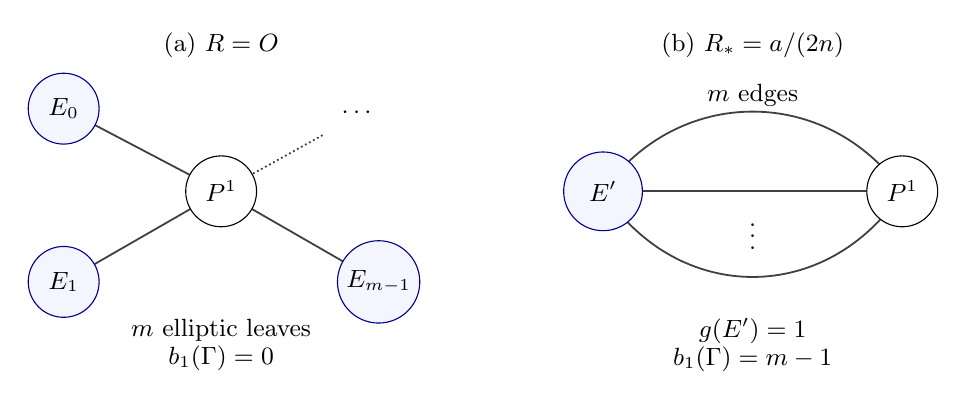
\begin{tikzpicture}[
  x=1cm,y=1cm,
  every node/.style={font=\small,inner sep=2pt},
  component/.style={draw,fill=white,circle,minimum size=9mm},
  elliptic/.style={component,draw=blue!55!black,fill=blue!4},
  edge/.style={draw=black!75,line width=.65pt}
]
  \node at (2.5,3.65) {\textup{(a)} $R=O$};
  \node at (9.25,3.65) {\textup{(b)} $R_*=a/(2n)$};

  \coordinate (rational) at (2.5,1.8);
  \coordinate (leafzero) at (.5,2.85);
  \coordinate (leafone) at (.5,.65);
  \coordinate (leaflast) at (4.5,.65);
  \draw[edge] (rational) -- (leafzero);
  \draw[edge] (rational) -- (leafone);
  \draw[edge] (rational) -- (leaflast);
  \draw[edge,densely dotted] (rational) -- (3.8,2.52);
  \node at (4.22,2.8) {$\cdots$};
  \node[component] at (rational) {$\mathbb P^1$};
  \node[elliptic] at (leafzero) {$E_0$};
  \node[elliptic] at (leafone) {$E_1$};
  \node[elliptic] at (leaflast) {$E_{m-1}$};
  \node[align=center] at (2.5,-.15)
    {$m$ elliptic leaves\\[-1pt] $b_1(\Gamma)=0$};

  \coordinate (emain) at (7.35,1.8);
  \coordinate (tail) at (11.15,1.8);
  \draw[edge] (emain) .. controls (8.3,3.15) and (10.2,3.15) .. (tail);
  \draw[edge] (emain) -- (tail);
  \draw[edge] (emain) .. controls (8.3,.35) and (10.2,.35) .. (tail);
  \node[fill=white,inner sep=1pt] at (9.25,1.33) {$\vdots$};
  \node[elliptic,minimum size=10mm] at (emain) {$E'$};
  \node[component] at (tail) {$\mathbb P^1$};
  \node at (9.25,3.02) {$m$ edges};
  \node[align=center] at (9.25,-.15)
    {$g(E')=1$\\[-1pt] $b_1(\Gamma)=m-1$};
\end{tikzpicture}
